\section{Data Analysis}
\label{Data Analysis}
All of our data goes here, straight up with no analysis.  If it is a figure, you need a figure name underneath and you must describe it in the following paragraph.  

If it is a table, you need to include a title above the table.  You must also describe the table before inserting it.  

\begin{figure}
\centering
\begin{subfigure}{.5\textwidth}
  \centering
  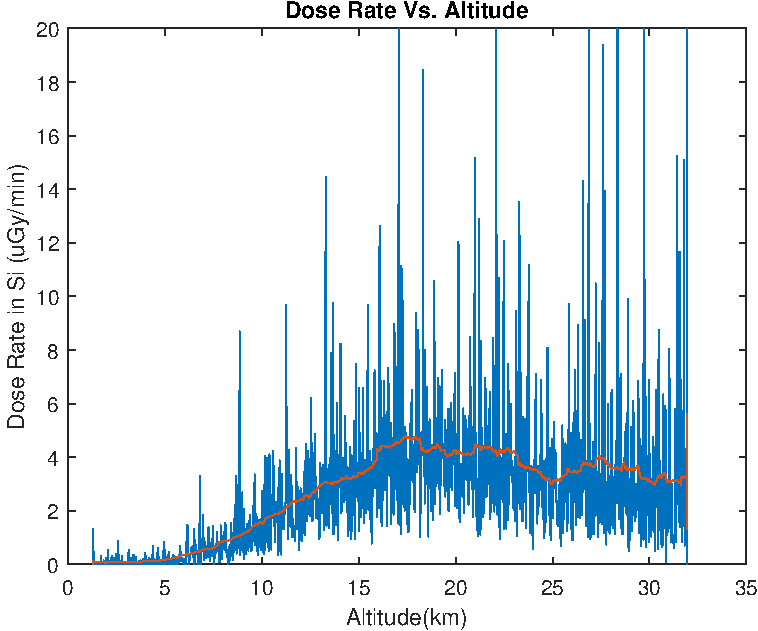
\includegraphics[scale=.5]{dva-cropped.pdf}
  \caption{Dose rate in silicon vs. altitude.}
  \label{fig:sub1}
\end{subfigure}%
\begin{subfigure}{.5\textwidth}
  \centering
  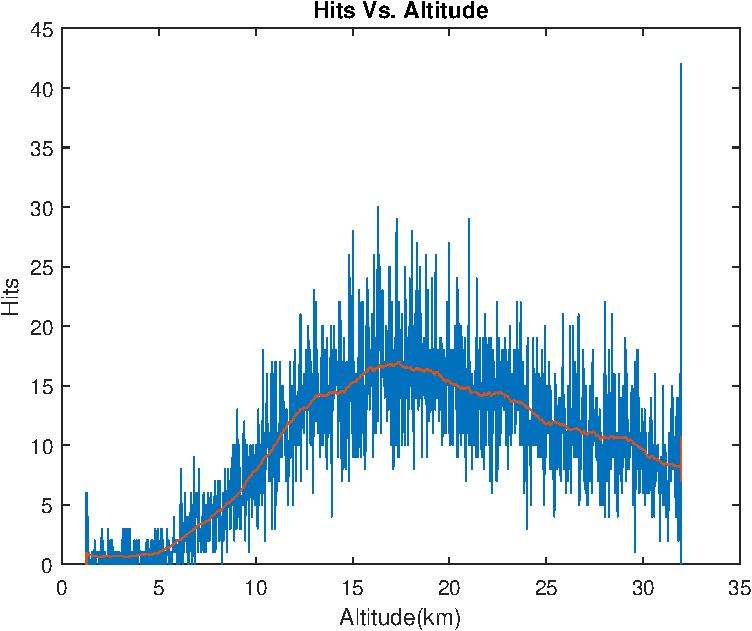
\includegraphics[scale=.5]{hva-cropped.pdf}
  \caption{Detector Hits vs. altitude.}
  \label{fig:sub2}
\end{subfigure}
\caption{Not sure what to put here yet.}
\label{fig:test}
\end{figure}

\begin{figure}[h]
\centering
\caption{Cluster Type Counts vs. altitude.}
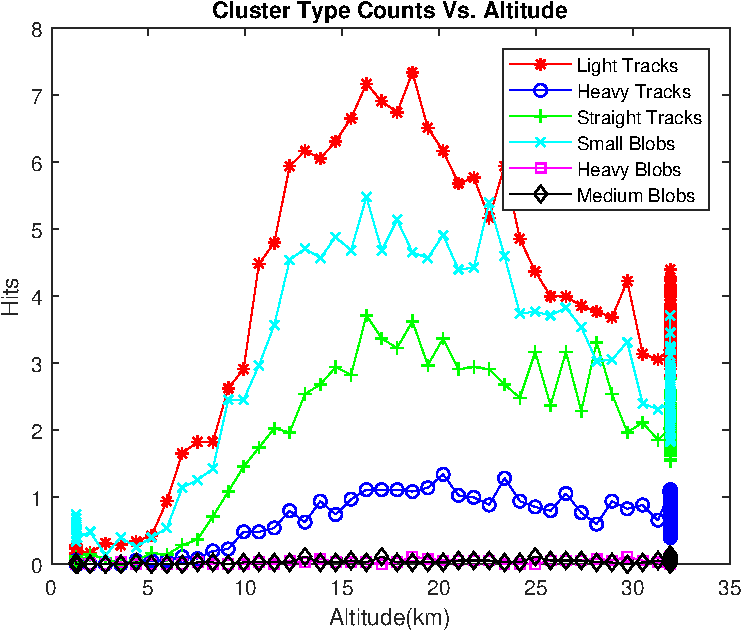
\includegraphics[scale=.5]{ctva-cropped.pdf}
\end{figure}
